\documentclass[tikz,border=12pt]{standalone}
% Estilo comum dos esquemas vetoriais das aulas da GA033.
\usepackage[T1]{fontenc}
\usepackage[utf8]{inputenc}
\usepackage{lmodern}
\usepackage{amsmath,amssymb}
\usetikzlibrary{arrows.meta,positioning,calc,fit,matrix,decorations.pathreplacing,backgrounds,shapes.geometric}
\definecolor{lnccblue}{HTML}{075AC0}
\definecolor{ink}{HTML}{242A31}
\definecolor{muted}{HTML}{647080}
\definecolor{lightblue}{HTML}{EFF5FC}
\definecolor{teal}{HTML}{197C83}
\definecolor{orange}{HTML}{BC6A16}
\tikzset{
  every node/.style={font=\sffamily\fontsize{15}{18}\selectfont,text=ink},
  box/.style={draw=lnccblue,line width=0.9pt,fill=lightblue,inner sep=9pt,align=center},
  flow/.style={-{Stealth[length=3mm,width=2mm]},draw=lnccblue,line width=1pt},
  point/.style={circle,draw=lnccblue,fill=white,line width=1.2pt,minimum size=3.2mm,inner sep=0pt},
  label/.style={font=\sffamily\fontsize{13}{16}\selectfont,text=muted},
  heading/.style={font=\sffamily\bfseries\fontsize{16}{19}\selectfont,text=lnccblue}
}
% Impede setas horizontais involuntariamente invertidas após editar os nós.
\newdimen\origemseta
\newdimen\destinoseta
\newcommand{\verificarsetadireita}[2]{%
  \pgfextractx{\origemseta}{\pgfpointanchor{#1}{east}}%
  \pgfextractx{\destinoseta}{\pgfpointanchor{#2}{west}}%
  \advance\origemseta by 4mm%
  \ifdim\destinoseta>\origemseta\else
    \PackageError{diagramas}{Conector sem espaco entre #1 e #2}{Afaste os nos antes de compilar.}%
  \fi
}

\begin{document}
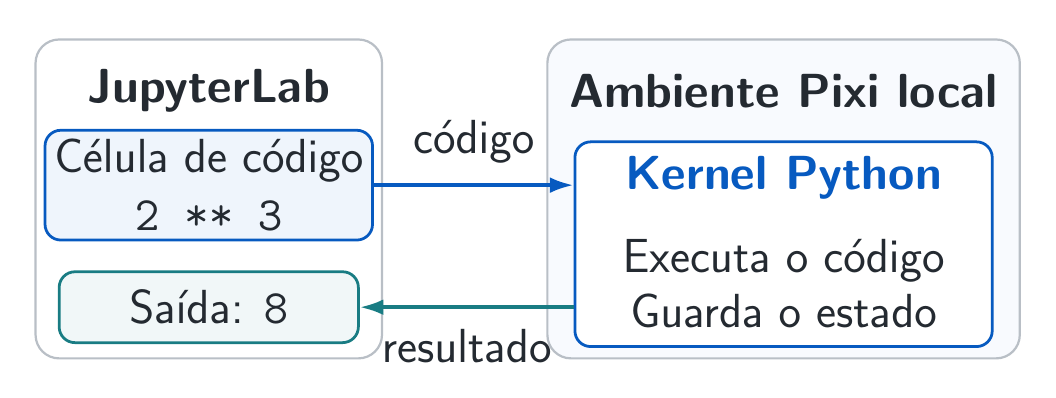
\begin{tikzpicture}[
  x=1cm,y=1cm,
  every node/.append style={font=\sffamily\fontsize{17}{21}\selectfont},
  painel/.style={draw=muted!45,rounded corners=3mm,line width=.8pt},
  celula/.style={draw=lnccblue,fill=lightblue,rounded corners=2mm,
    line width=1pt,align=center,minimum width=3.8cm,minimum height=.9cm},
  seta/.style={-{Latex[length=3mm,width=2mm]},draw=lnccblue,line width=1.3pt}
]
\path[use as bounding box] (-.1,-1.8) rectangle (12.6,2.55);
\draw[painel] (0,-1.65) rectangle (4.4,2.4);
\node[text=ink,font=\sffamily\fontsize{18}{22}\selectfont\bfseries] at (2.2,1.75) {JupyterLab};
\node[celula] (codigo) at (2.2,.55) {Célula de código\\\texttt{2 ** 3}};
\node[celula,draw=teal,fill=teal!6] (saida) at (2.2,-1.0) {Saída: \texttt{8}};

\draw[painel,fill=lightblue!45] (6.5,-1.65) rectangle (12.5,2.4);
\node[text=ink,font=\sffamily\fontsize{18}{22}\selectfont\bfseries] at (9.5,1.75) {Ambiente Pixi local};
\node[draw=lnccblue,fill=white,rounded corners=2mm,line width=1pt,
  minimum width=5.3cm,minimum height=2.6cm] (kernel) at (9.5,-.2) {};
\node[text=lnccblue,font=\sffamily\fontsize{18}{22}\selectfont\bfseries] at (9.5,.65) {Kernel Python};
\node[align=center,text=ink,text width=4.7cm,
  font=\sffamily\fontsize{16}{20}\selectfont] at (9.5,-.7) {Executa o código\\Guarda o estado};

\verificarsetadireita{codigo}{kernel}
\verificarsetadireita{saida}{kernel}
\draw[seta] (codigo.east) -- (kernel.west |- codigo.east)
  node[midway,above=4pt,text=ink,font=\sffamily\fontsize{16}{20}\selectfont] {código};
\draw[seta,draw=teal] (kernel.west |- saida.east) -- (saida.east)
  node[midway,below=4pt,text=ink,font=\sffamily\fontsize{16}{20}\selectfont] {resultado};
\end{tikzpicture}
\end{document}
